Er is een speciale hidden feature in Windows die je toegang geeft tot bijna 200 configuratie items. Deze wordt dan ook de God Mode genoemd. Toegang tot deze enorme collectie aan configuratie items is simpel te verzorgen. Maak op je Desktop een lege map aan, hernoem deze naar: GodMode.{ED7BA470-8E54-465E-825C-99712043E01C} en nadat je enter hebt gegeven verander het icon van de map.

\begin{minipage}[t]{\linewidth}
\raggedright
\adjustbox{valign=t}{%
	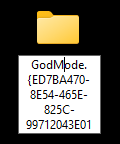
\includegraphics[width=76pt]{godmode-map.png}%
	\hspace{1cm}%
	
\includegraphics[width=93pt]{godmode-icon.png}%
}
\end{minipage}

Dubbel klik op het nieuwe icoon.

\begin{minipage}[t]{\linewidth}
\raggedright
\adjustbox{valign=t}{%
	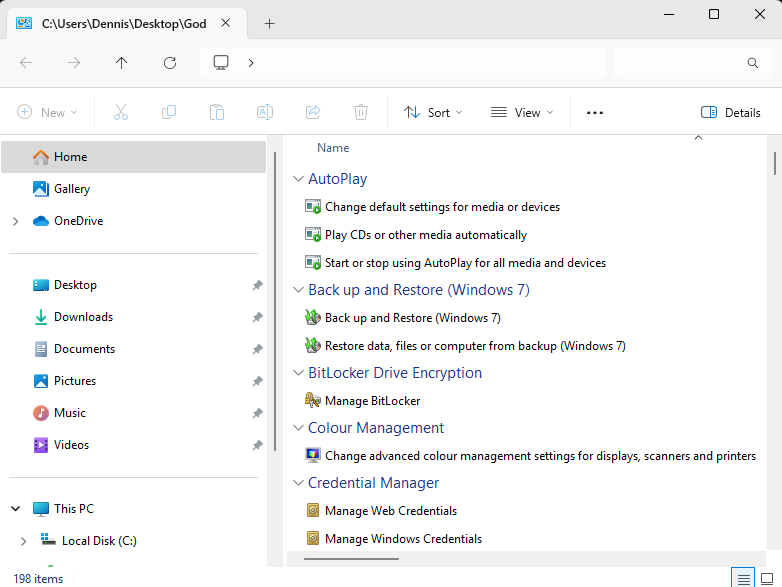
\includegraphics[width=0.99\linewidth]{godmode.png}%
}
\end{minipage}
